%!TEX root = ../thesis.tex
% ******************************* Thesis Appendix B ********************************

\chapter{The Catastrophe Machine}
\label{app:catasrophe}


\ifpdf
\graphicspath{{Appendix3/Figs/Raster/}{Appendix3/Figs/PDF/}{Appendix3/Figs/}}
\else
\graphicspath{{Appendix3/Figs/Vector/}{Appendix3/Figs/}}
\fi

\definecolor{Gray}{gray}{0.92}

\newcolumntype{P}[2]{%
	>{\begin{turn}{#1}\begin{minipage}{#2}\small\raggedright\hspace{0pt}}l%
			<{\end{minipage}\end{turn}}%
}
\newcolumntype{R}[2]{%
	>{\columncolor{Gray}}
	>{\begin{turn}{#1}\begin{minipage}{#2}\small\raggedright\hspace{0pt}}l%
			<{\end{minipage}\end{turn}}%
}
\newcolumntype{a}{>{\columncolor{Gray}}c}



The Zeeman's catastrophe machine is a historically important example to illustrate critical transitions governed by a cusp bifurcation. It can be easily constructed and allows to showcase the effect of control parameters towards abrupt shifts. Since it is governed by classical laws of mechanics, it is also possible to reproduce its dynamics and to predict its stability behaviour. In addition, the Catastrophe Machine is a powerful tool for teaching: it is among the simplest (closed) systems that exhibit tipping and hysteresis, which can be shown simply and intuitively. More advanced machines can be used to illustrate different critical transitions \citep{woodcock1976higher} or the appearance of chaotic behaviour when multiple nonlinear systems are coupled \citep{nagy2013zeeman}.

Because of its benefits (didactics, intuition, manipulation, modelling), the catastrophe machine is a nice tool to have. Thanks to the support of the LCSB maintenance team, I constructed a simple machine (described in details below) and a more advanced one, that shows routes to chaos. The photographs in this section depict our catastrophe machine during practical exercises.




\tocless\section{What is the Catastrophe Machine}

The Catastrophe machine was invented by E. C. Zeeman as a toy for illustrating the at-that-time new Catastrophe Theory \citep{poston1973zeeman,zeeman1979catastrophe}. It consists on a wheel governed by a couple of elastics, connected to the wheel by a pivot; one elastic is fixed to a pin, while the other can be controlled by the user. Everything is set on a board, see Fig. \ref{0a}.


\begin{figure}[h]
	\centering
	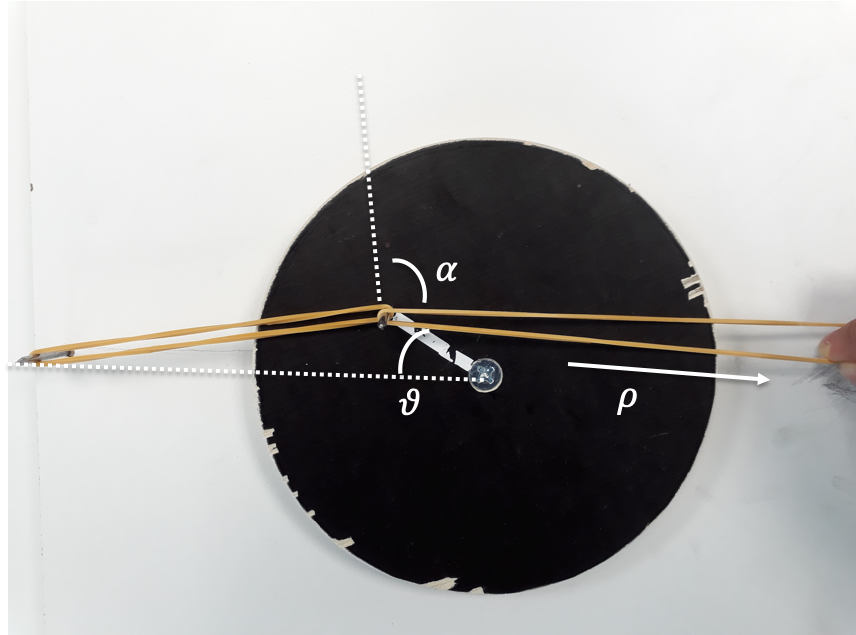
\includegraphics[width=0.42\linewidth]{sketch}
	\caption{\small The catastrophe machine is composed by wheel and elastics, one of which is fixed by a pin while the other is held by the user. The angle $\theta$ is considered as state variable; $\alpha$ represents the reciprocal position of the two elastics; $\rho$ is the force exerted by the user (forcing); it also accounts for the friction, that is always opposing the movement. In order for the machine to move, the friction should not be too high \citep{poston1979catastrophe}).}
	\label{0a}
\end{figure}


The machine empirically exhibits sudden shifts: if the second elastic is stretched past a threshold, the wheel turns abruptly. Hysteresis is also observed when the second elastic is relaxed: to tip back, it must shrink past the point of the first tipping (Fig. \ref{fig:CM_eamples}a--d). The machine shows the same qualitative behaviour regardless of wheel radius, un-stretched elastics lengths and distance from pin to wheel centre. This is a``structural stability'' property: changes in parameters make no essential qualitative difference \citep{poston1979catastrophe}. Hence, the catastrophe machine is a perfect toy model to study critical transitions: it is controllable, it is possible to calculate its potential and to study different configurations leading to similar qualitative behaviours \citep{Thom2554}. \\

\begin{figure}[h]
	\centering
	\begin{minipage}[c]{0.22\textwidth}
		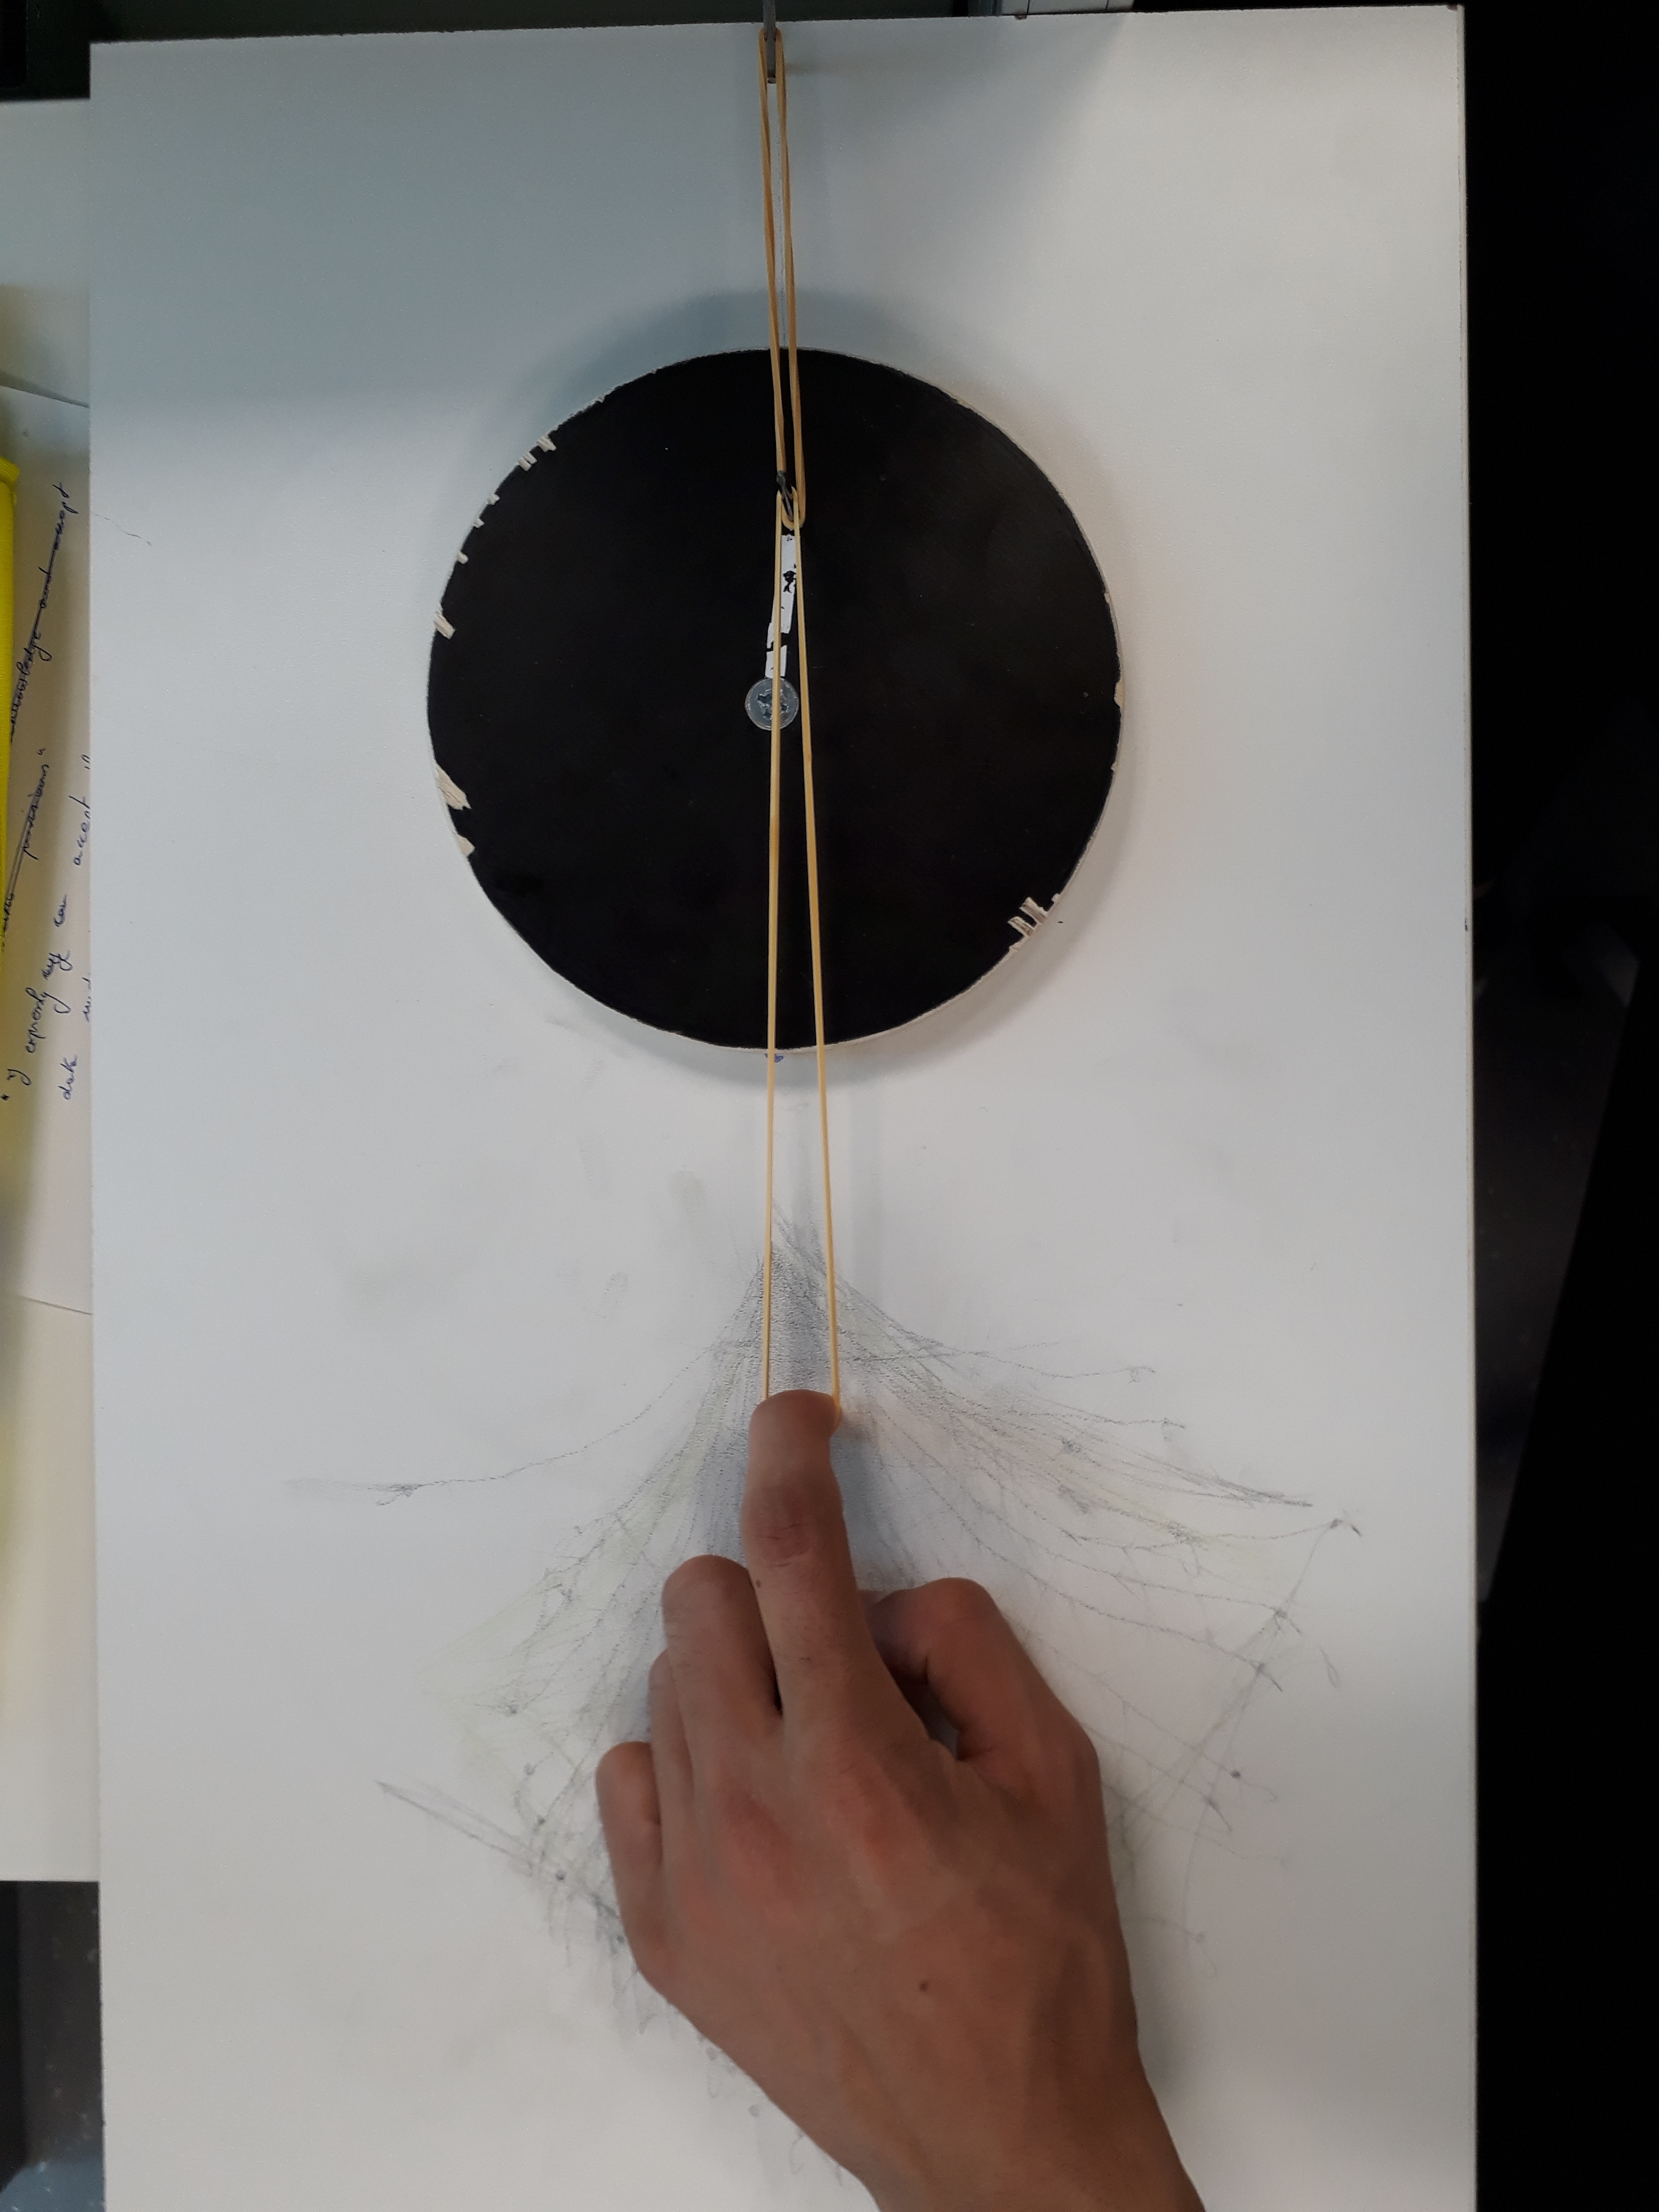
\includegraphics[width=\linewidth]{mac1.jpg}
		\renewcommand{\figurename}{Fig.}
		\caption*{(a)}
	\end{minipage}
	\hspace{0.1cm}
	\begin{minipage}[c]{0.22\textwidth}
		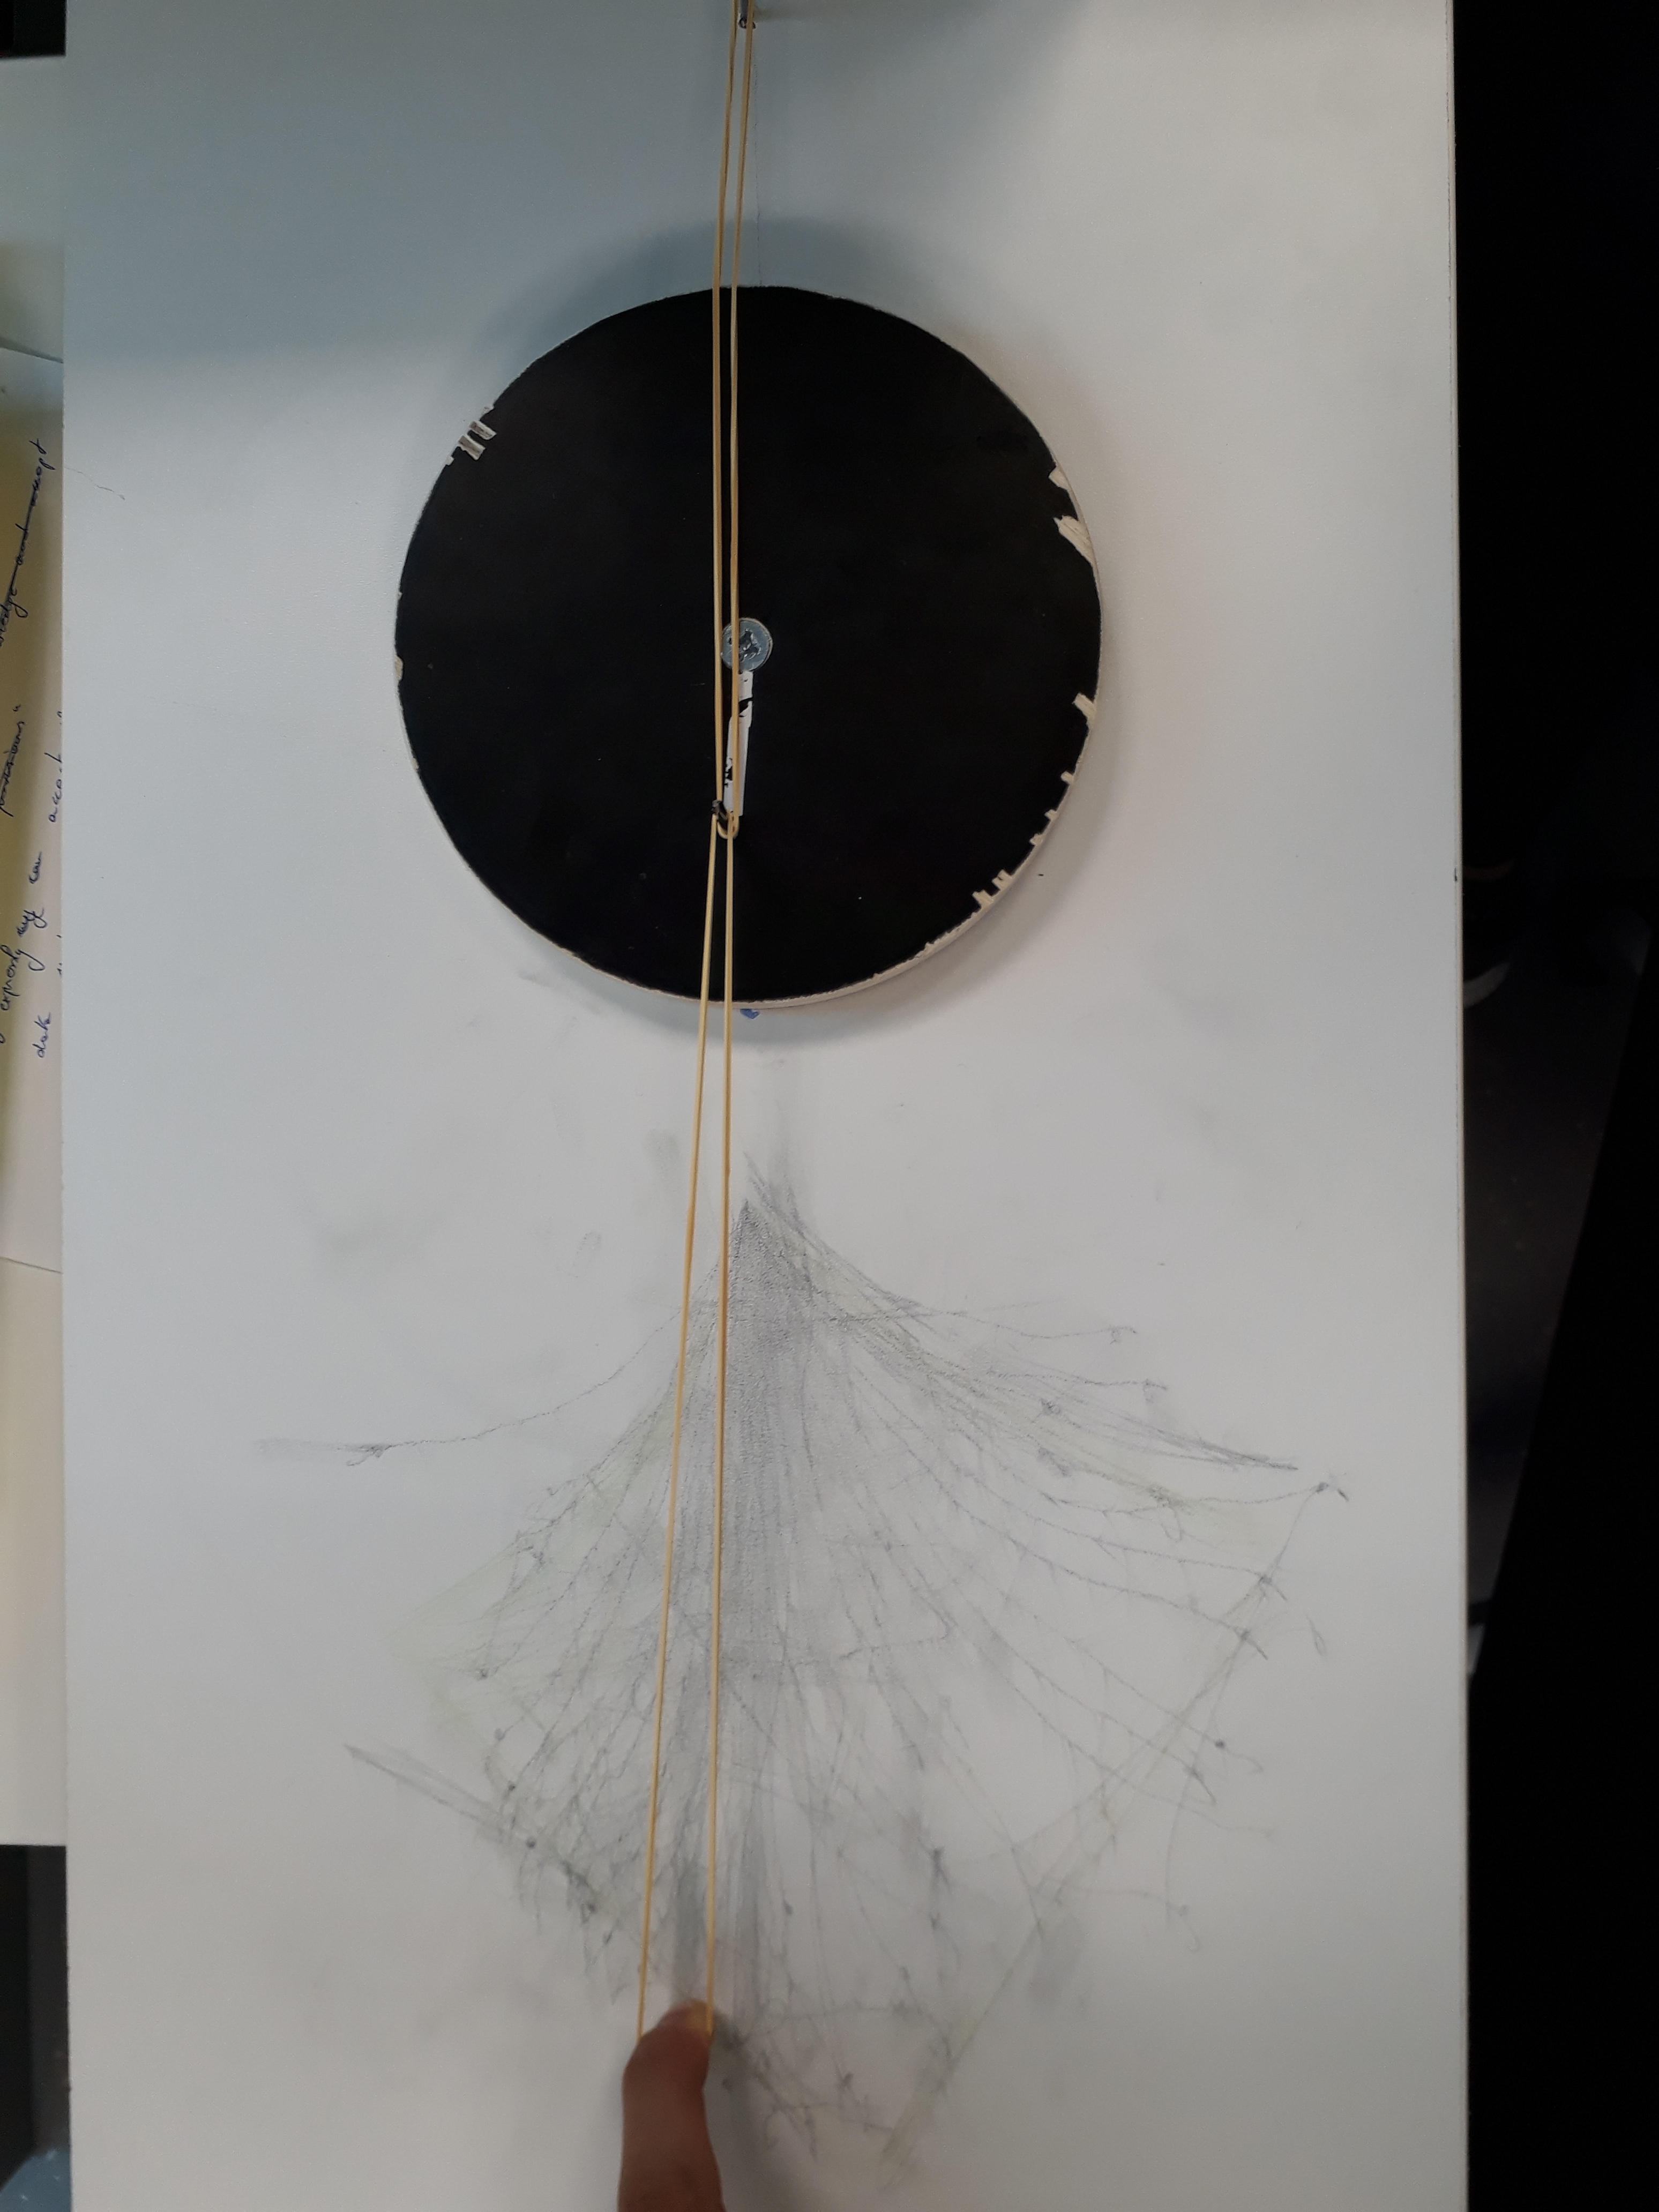
\includegraphics[width=\linewidth]{mac2.jpg}
		\renewcommand{\figurename}{Fig.}
		\caption*{(b)}
	\end{minipage} 
	\hspace{0.1cm}
	\begin{minipage}[c]{0.22\textwidth}
		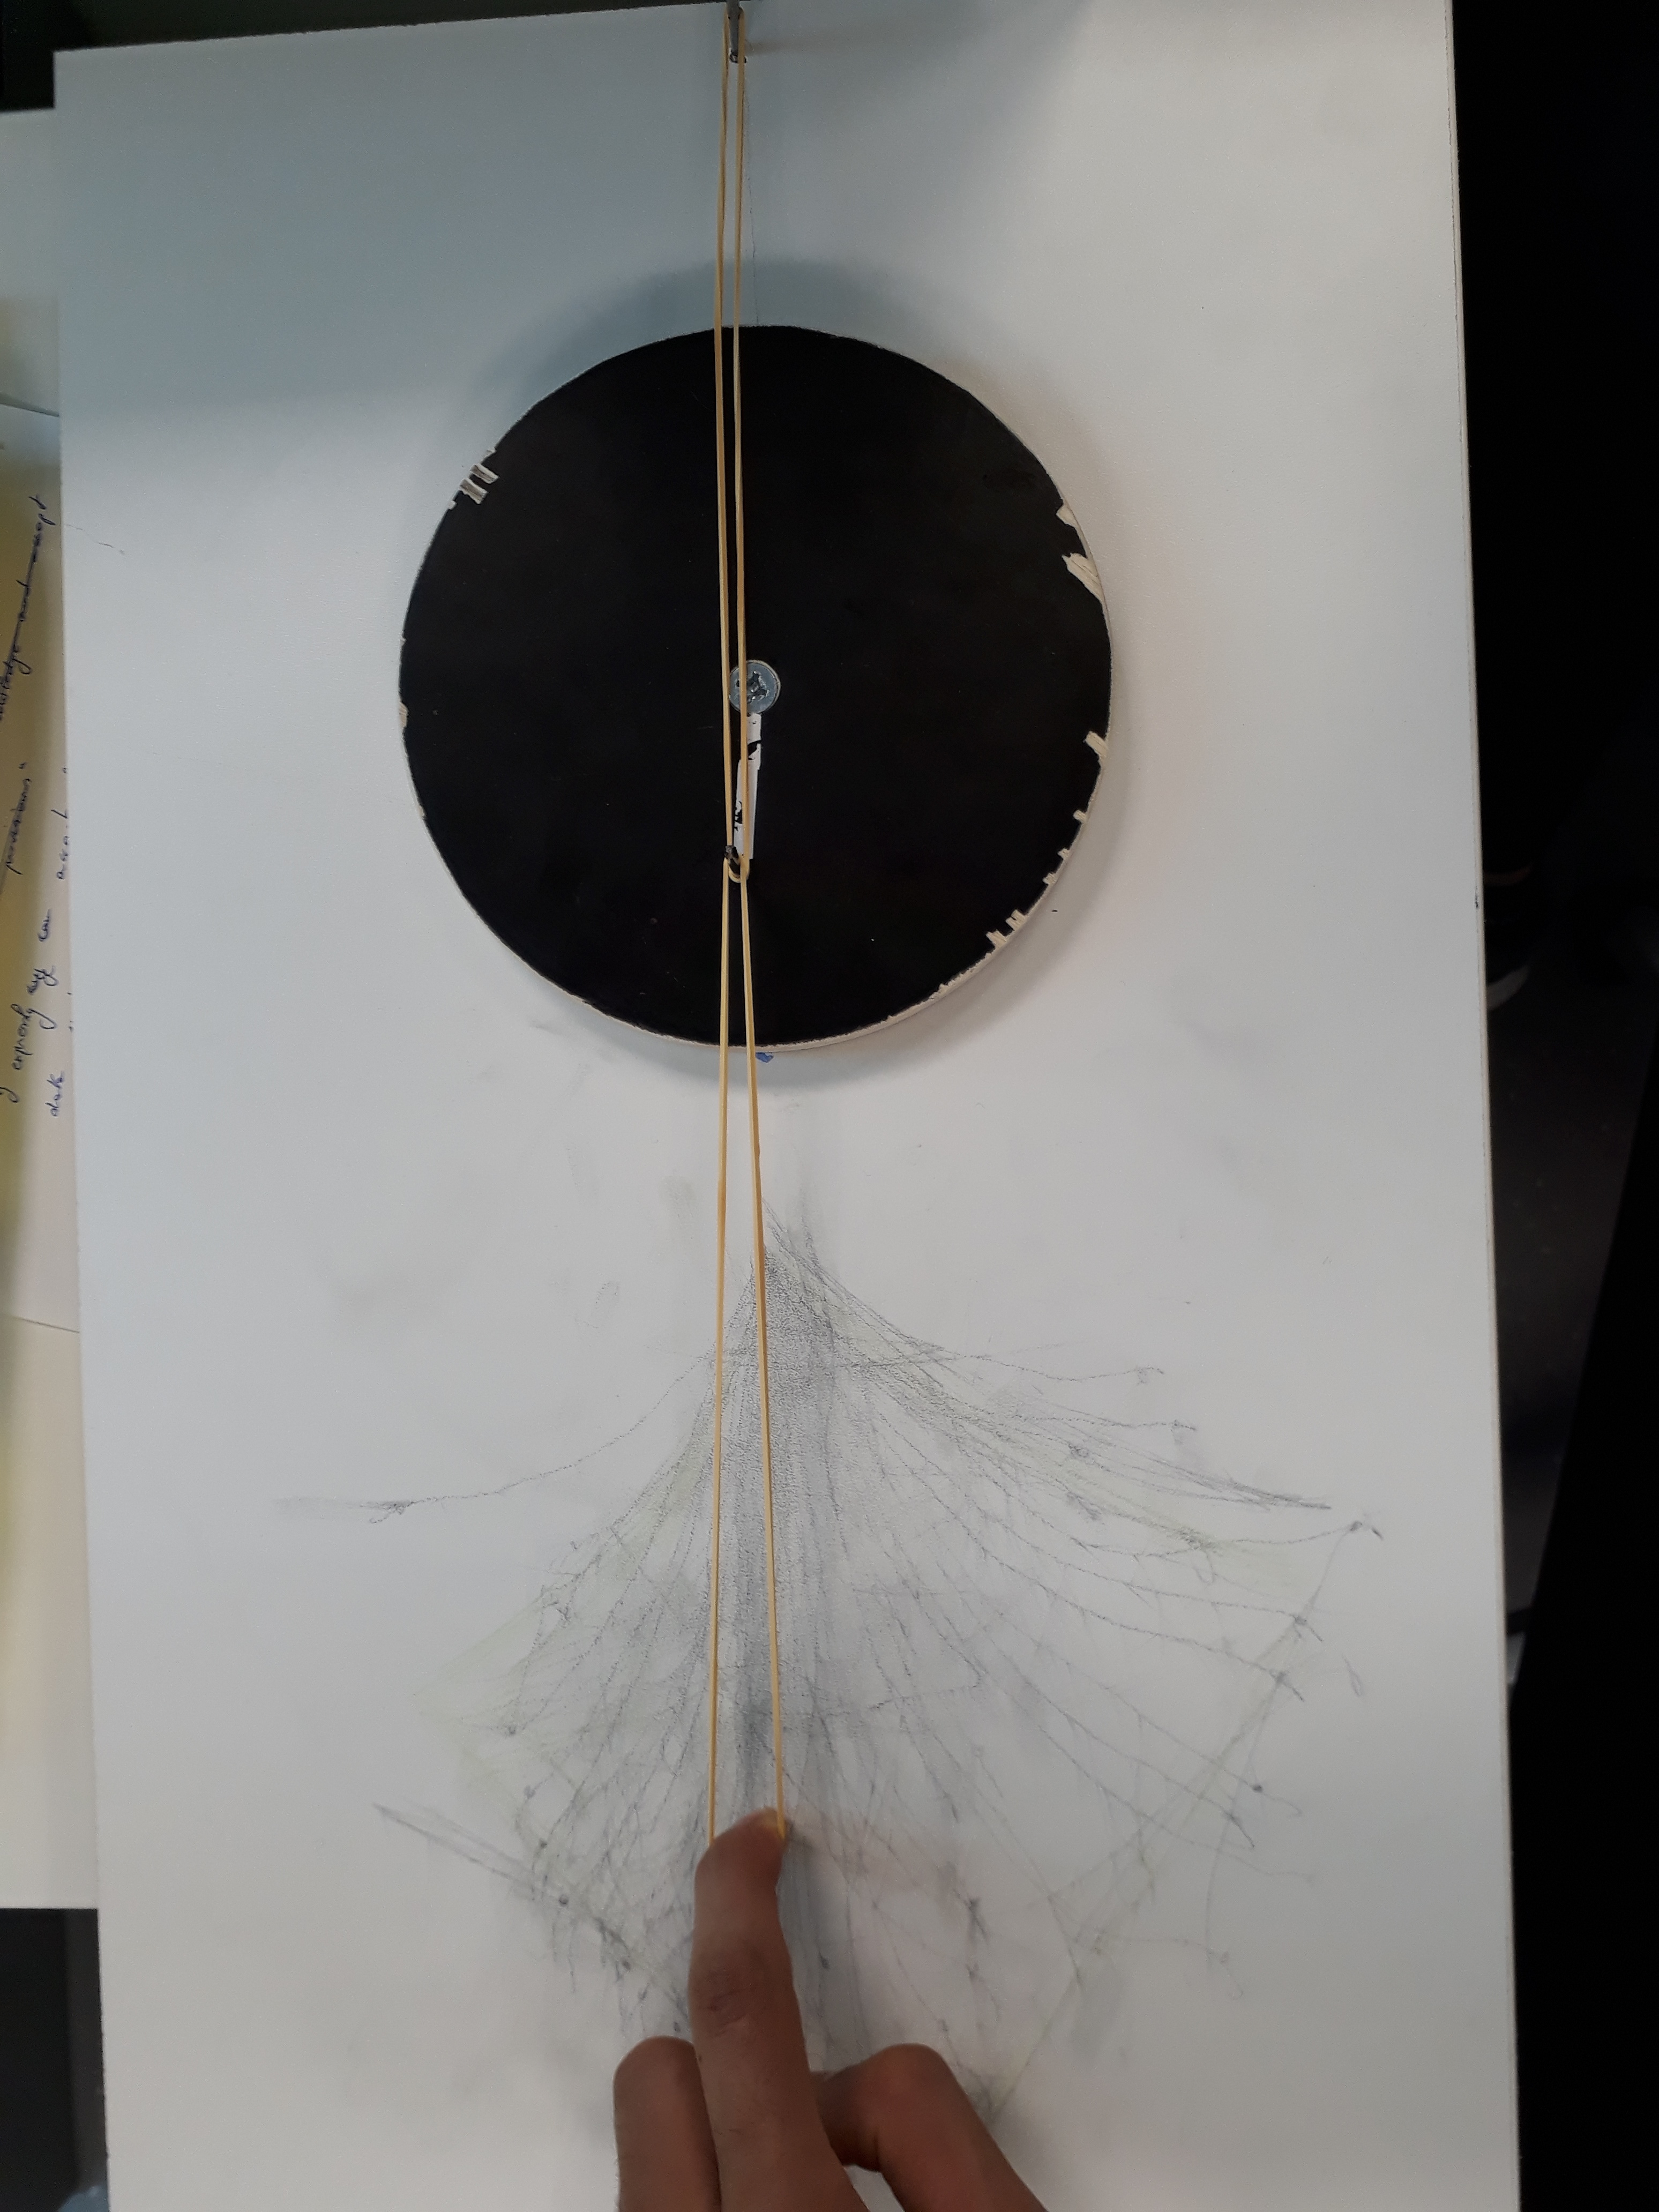
\includegraphics[width=\linewidth]{mac3.jpg}
		\renewcommand{\figurename}{Fig.}
		\caption*{(c)}
	\end{minipage}
	\hspace{0.1cm}
	\begin{minipage}[c]{0.22\textwidth}
		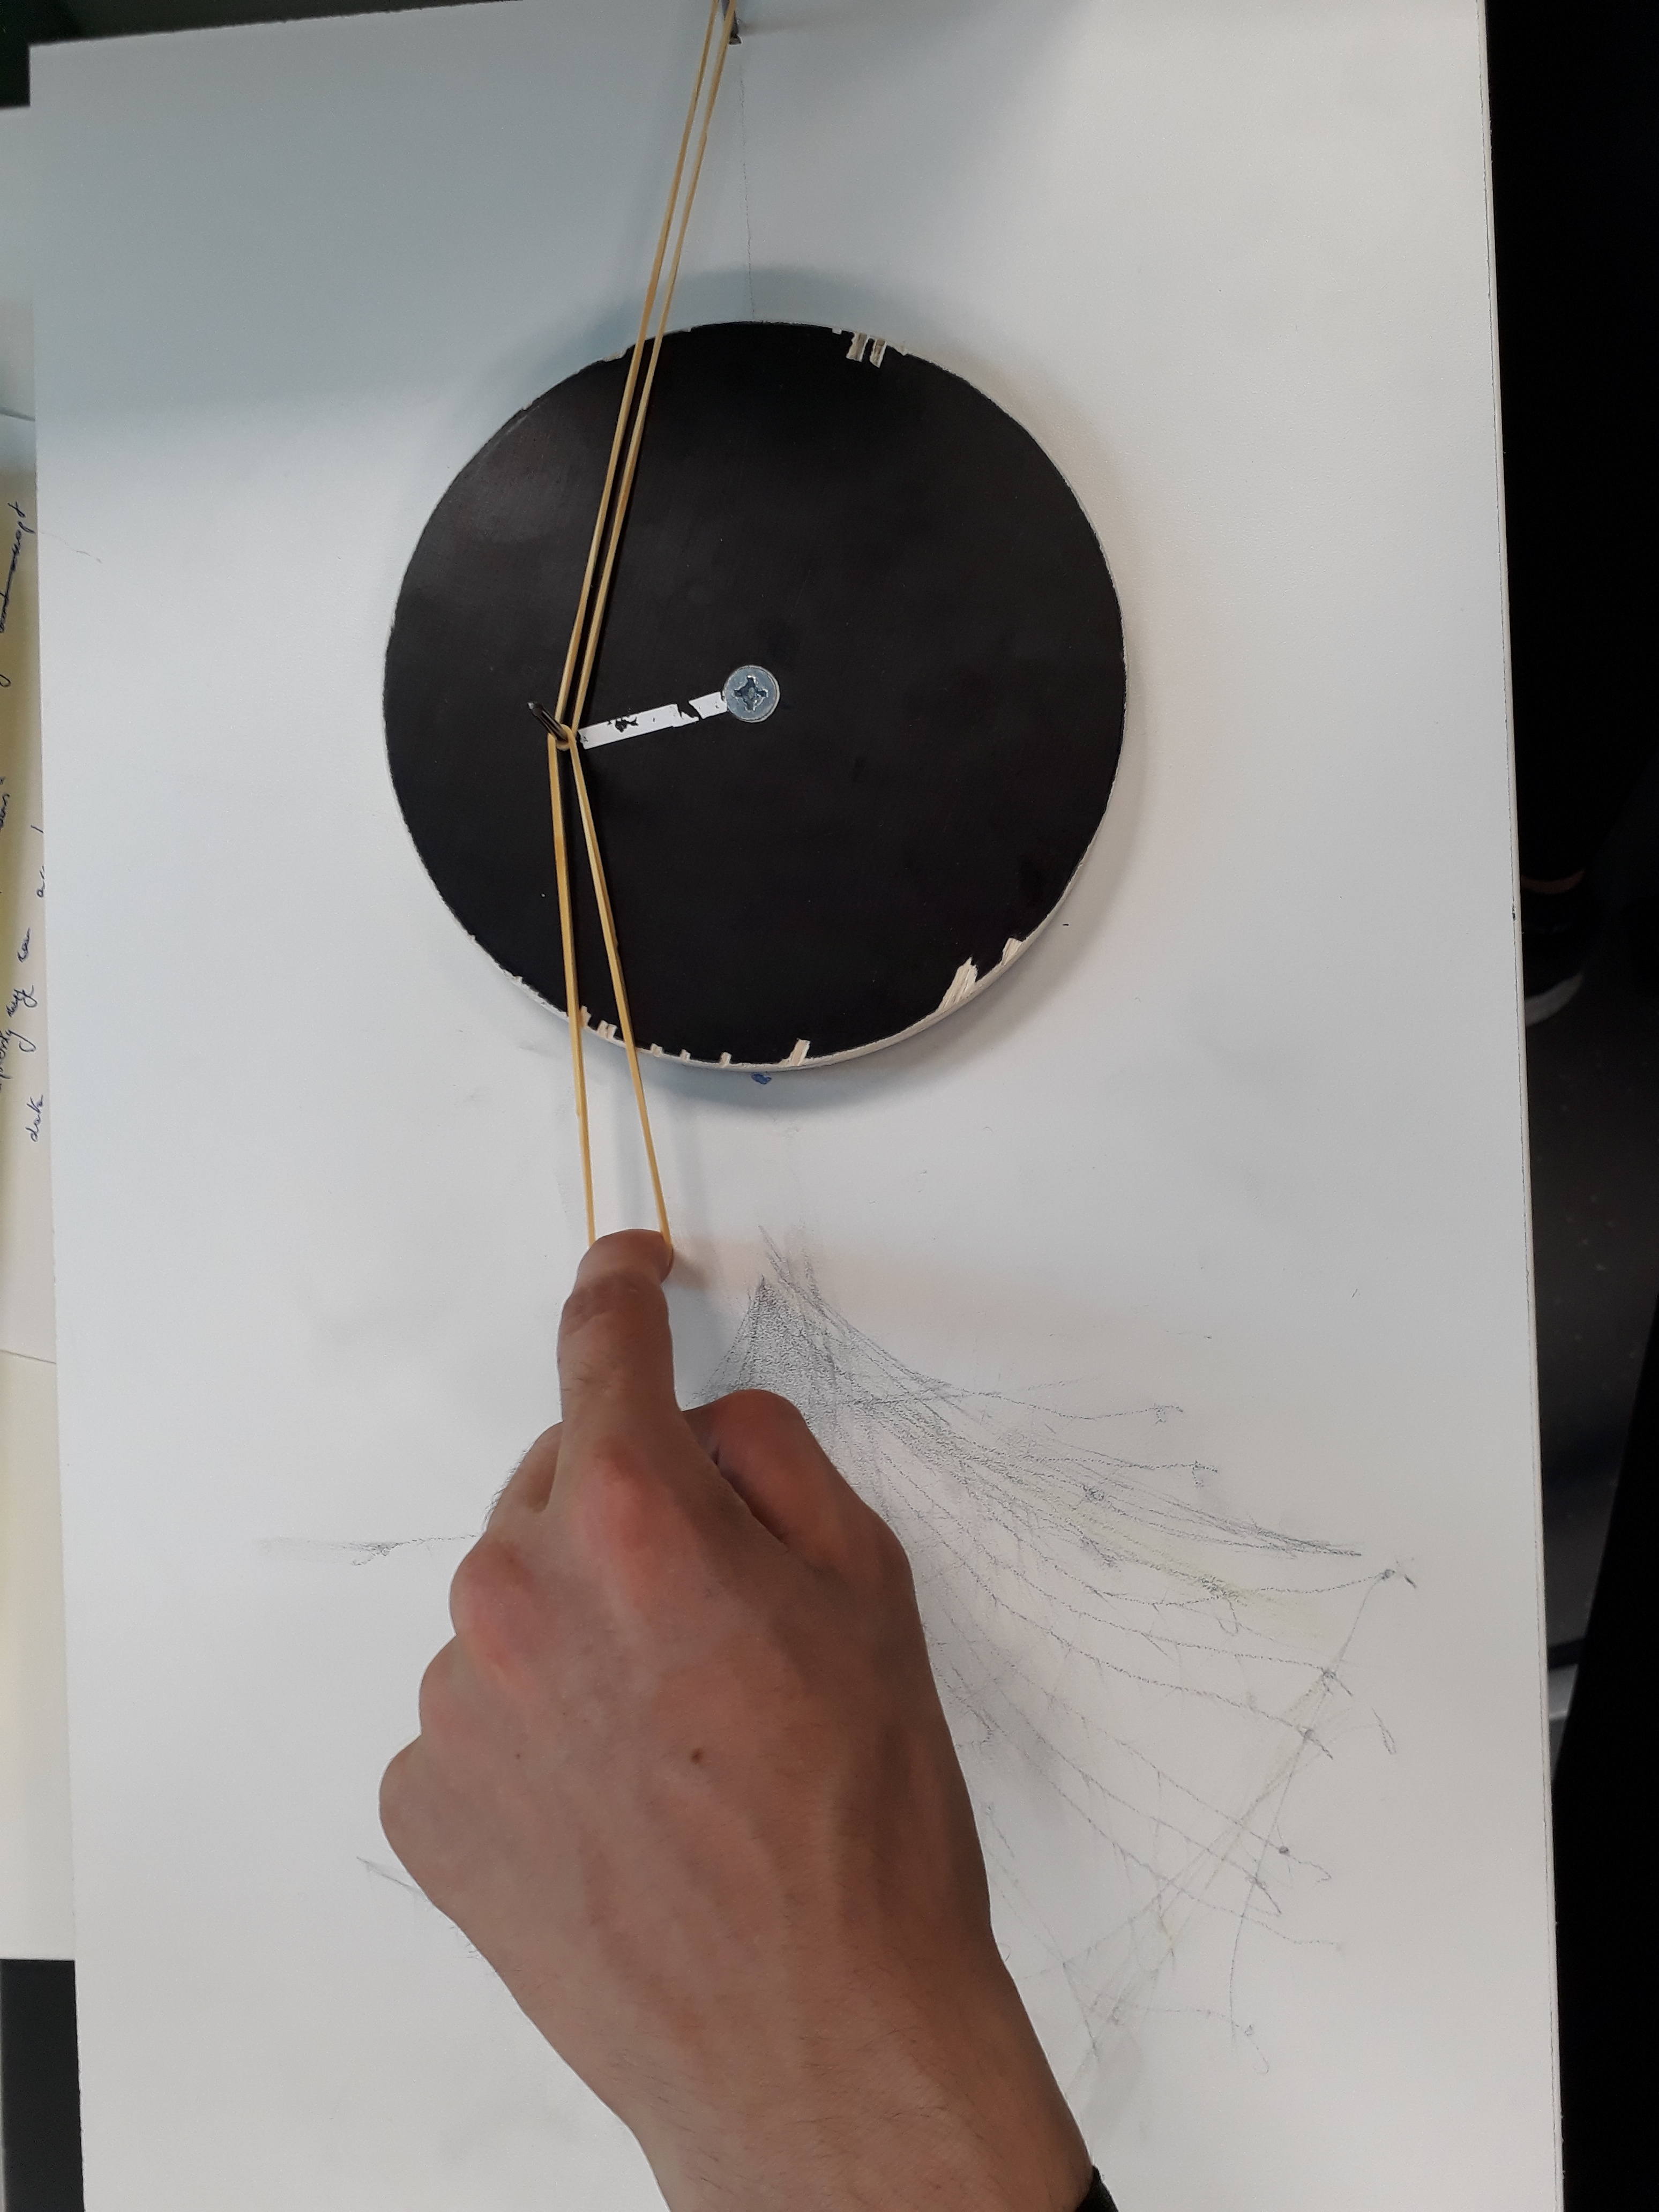
\includegraphics[width=\linewidth]{mac4.jpg}
		\renewcommand{\figurename}{Fig.}
		\caption*{(d)}
	\end{minipage}
	\caption{\small Tipping and hysteresis can be observed in the evolution of the system (from left to right). \textbf{a:} The machine is at equilibrium: a small forcing is not enough to move it. \textbf{b:} the forcing overcomes a threshold, and the wheel turns rapidly to a new equilibrium. \textbf{c:} such equilibrium is kept stable by the friction; if we let the elastic shrink, the wheel does not return to the initial position by passing through the previous point. \textbf{d:} when a second threshold is passed, the wheelturns back to the first equilibrium. A video animation is provided, see link in Appendix \ref{app:animations}}
	\label{fig:CM_eamples}
\end{figure}




\tocless\section{Solving the stability problem}

As anticipated above, the state variable is identified by the angle $\theta$, while the parameter $\alpha$ represents the ratio between the angle spanned by the second elastic w.r.t. the $x$ axis and $\theta$; $\rho$ is the forcing (see Fig. \ref{0a}). To study the stability of the machine, it is sufficient to look at its potential. It is possible to study the Lagrangian \citep{nagy2013zeeman} or, in the simple static case, to consider the forces acting on the system (see Fig. \ref{vector}) and then integrate. We follow the second approach. Let us define:
\begin{itemize}
	\item OP = 1. It is the wheel radius; its value is set to unitary measure without loss of generality.
	\item $L_1$ and $L_2$: lengths at rest of the two elastics.
	\item  $F_{\text{el1}}$ and $F_{\text{el2}}$ are, respectively, the elastic forces stored by elastic 1 and 2; they follow Hook's law $F_{el} = -k_{\text{el}} \, \Delta L$. $k_{\text{el}}$ is the elastic constant.
	\item $T_m$ represents the machine's torque.
\end{itemize}
Let us also employ the long distance approximation: AB is almost parallel to the $x$ axis (to select order of expansions for $\theta$).

\begin{figure}[h!]
	\centering
	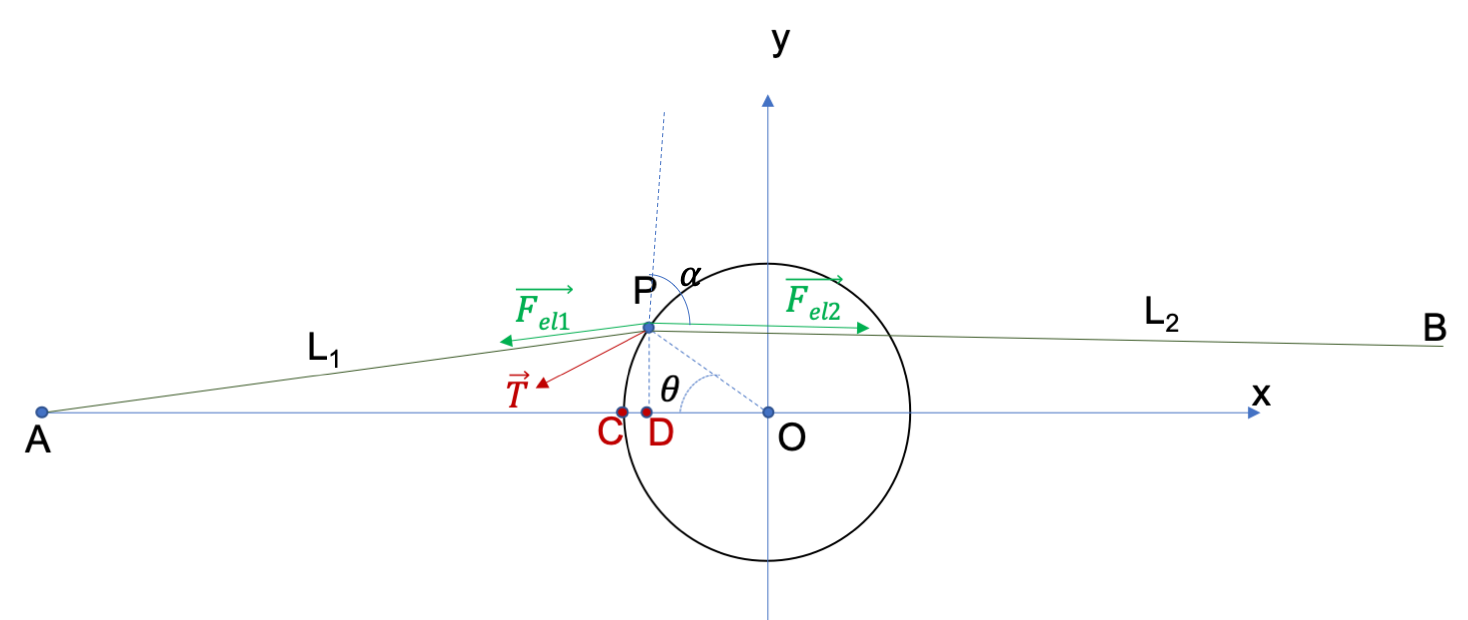
\includegraphics[width=0.7\linewidth]{vectors}
	\caption{\small Sketch of the forces acting on the machine.}
	\label{vector}
\end{figure}

By applying simple mechanic considerations, we first estimate the potential term related to the elastic forces at rest. Start by:
\begin{equation*}
	F_{\text{el1}} = -k_{\text{el}}  \cdot CD = k_{\text{el}} (1-\cos\theta) \, .
\end{equation*}
Considering the small angles approximation helping to truncate the Taylor expansion up to $O(\theta^3)$,
\begin{equation*}
	T \simeq F_{\text{el1}} \, \sin\theta = k_{\text{el}} (1-\cos\theta)\sin\theta \simeq k_{\text{el}} \left(1-1+\frac{\theta^2}{2} \right)\theta = k_{\text{el}} \, \frac{\theta^3}{2} + O(\theta^4) \, .
\end{equation*}
Hence, the potential is 
\begin{equation*}
	V(\theta) \propto k_{\text{el}} \, \theta^4 + \text{perturbations} \, .
\end{equation*}

The ``perturbations'' are added to account for whatever moves the configuration from its resting state. We thus estimate the perturbative terms with respect to additional parameters:
\begin{itemize}
	\item $\alpha$ quantifies the shift from the ``$AB \parallel x$'' assumption. By applying a Taylor expansion to the elastic force\footnote{$F(\theta + \Delta \theta) \simeq F(\theta) + \frac{dF}{d \theta}(\theta - 0) + O(\theta^2)$; if we assume (simplest form) that $F$ is linearly dependent on $\theta$ (ansatz, for small angles) then we get $F(\theta + \Delta \theta) \simeq F(\theta) + \alpha \theta $} we get (in the simplest, linear case) $F_{\text{pert}} \propto \alpha \theta$. 
	\item $\rho$ is directly the exerted force minus the friction.
\end{itemize}

As a consequence, the potential is:
\begin{equation}
	V(\theta) \propto \theta^4 - \alpha \theta^2 + \rho \theta \, .
	\label{eq:cm_potential}
\end{equation}

We can now play with this potential which is, up to numerical constants, the same one obtained using Langrangian methods \citep{poston1979catastrophe}. Numerical constants are neglected for two reasons: a) to concentrate on the effect of the parameters on the stability landscape, b) we here focus on qualitative predictions, therefore it is unnecessarily complex to take constants into account as the final result is independent on such details \citep{Thom2554}. 




\tocless\subsection{Analysis of the potential}
Depending on the parameters values, the potential takes different shapes underlying different stability properties. This section studies the effect of bending parameter $\alpha$ and tilting parameter $\rho$ on the potential and on its associated vector field $f(\theta, \bar{p}) = -\frac{dV(\theta, \bar{p})}{d \theta}$, $\bar{p}$ being the parameter set. \\

\tocless\subsubsection{Bending parameter $\alpha$}
First, focus on the effect of $\alpha$ alone. It is called ``bending parameter'', as it describes how the second elastic is bended compared to $\theta$. In addition, $\alpha$ has a bending effect on the potential (see Fig. \ref{fig:cm_bending}, right). Set $\rho = 0$ and consider :
\begin{equation}
	V(\theta) = \theta^4 - \alpha \theta^2
\end{equation}
and 
\begin{equation}
	f(\theta) = 4 \, \theta^3 - 2 \, \alpha \theta \, .
	\label{eq:potalpha}
\end{equation}
$\alpha$ is akin to the control parameter of a supercritical pitchfork bifurcation (Sec~\ref{app:supercr}) governing the bistability and the degree of hysteresis of the system, namely the possibility to develop smooth (low alpha) or critical transitions (high alpha). In fact, Eq. \ref{eq:potalpha} represents the normal form of a vector field associated to a supercritical pitchfork bifurcation (also compare Fig. \ref{fig:cm_bending} left with Fig. \ref{fig:superpitch_diagram}).

\begin{figure}[h]
	\centering
	\begin{minipage}[c]{0.48\textwidth}
		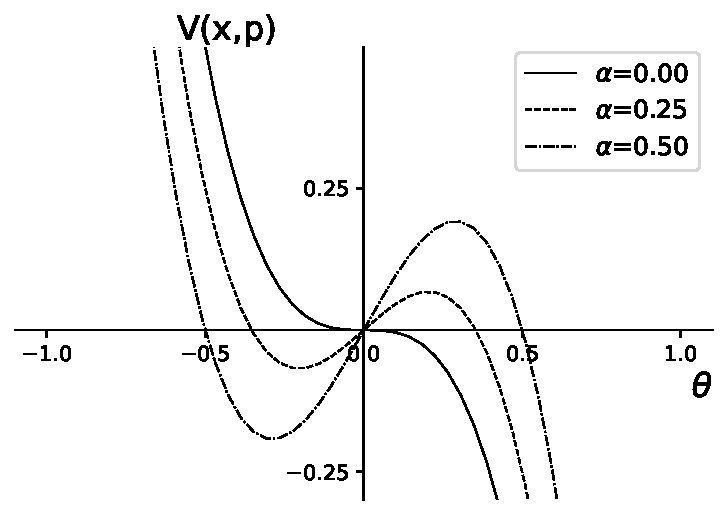
\includegraphics[width=\linewidth]{cat_mac_v}
		\renewcommand{\figurename}{Fig.}
	\end{minipage}
	\hspace{0.05cm}
	\begin{minipage}[c]{0.48\textwidth}
		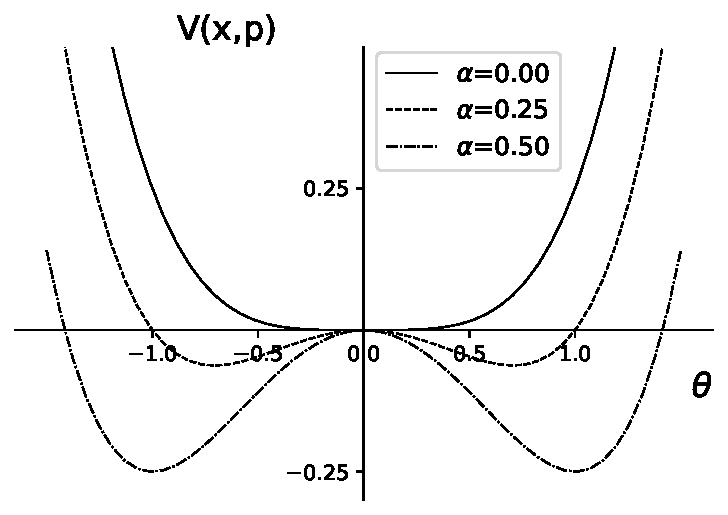
\includegraphics[width=\linewidth]{cat_mac_p}
		\renewcommand{\figurename}{Fig.}
	\end{minipage} 
	\caption{\small \textbf{Left:} $f(\theta)$ for various steady-state values of $\alpha$. If the bending parameter is augmented from zero to any other value, the vector field is deformed from being monotonous to having three different regions of monotonicity. \textbf{Right:} when $\alpha$ increases, the potential goes from a single equilibrium point to three, of which two are stable and the latter is unstable. The system is develops bistability: it is now susceptible to undergo critical transitions. The process is exactly analogous to a pitchfork bifurcation, Sec~\ref{app:supercr}.}
	\label{fig:cm_bending}
\end{figure}



\tocless\subsubsection{Tilting parameter $\rho$}
$\rho$ is termed ``tilting'' because it tilts the potential, see Fig. \ref{fig:cm_tilting}. To empathize what happens to the equilibria, let us fix $\alpha = 1$ to be in a bistable configuration. Then, study:
\begin{equation}
	V(\theta) = \theta^4 - \theta^2 + \rho \theta
\end{equation}
and 
\begin{equation}
	f(\theta) = 4 \, \theta^3 - 2 \,  \theta + \rho \, .
	\label{eq:potrho}
\end{equation}
Increasing values of $\rho$ cause the critical transition (provided that the system was already bistable), as one equilibrium suddenly loses stability and the other is pushed onto an alternative one. This follows the typical phenomena related to a fold catastrophe (saddle-node bifurcation, Sec~\ref{subsec:fold}). In fact, in the neighbourhood of the second equilibrium, the vector field can be expanded in the normal form of a fold ($f_{\text{local}} \simeq - \rho - \theta ^2$).\\


\begin{figure}[h]
	\centering
	\begin{minipage}[c]{0.48\textwidth}
		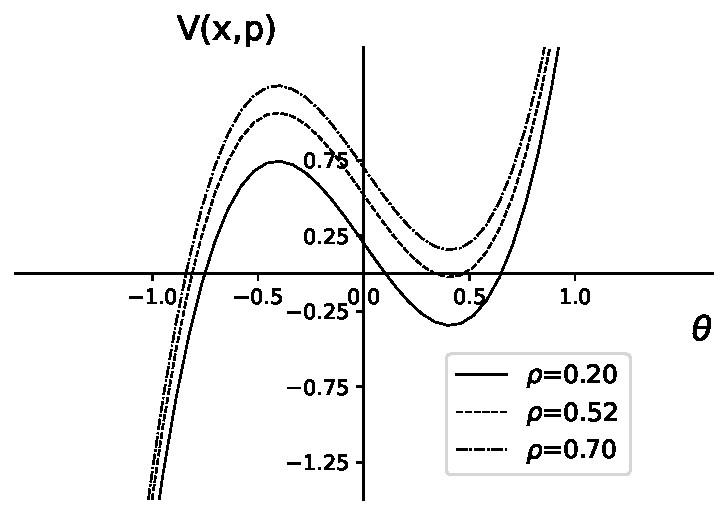
\includegraphics[width=\linewidth]{cat_mac_v_tilt}
		\renewcommand{\figurename}{Fig.}
	\end{minipage}
	\hspace{0.05cm}
	\begin{minipage}[c]{0.48\textwidth}
		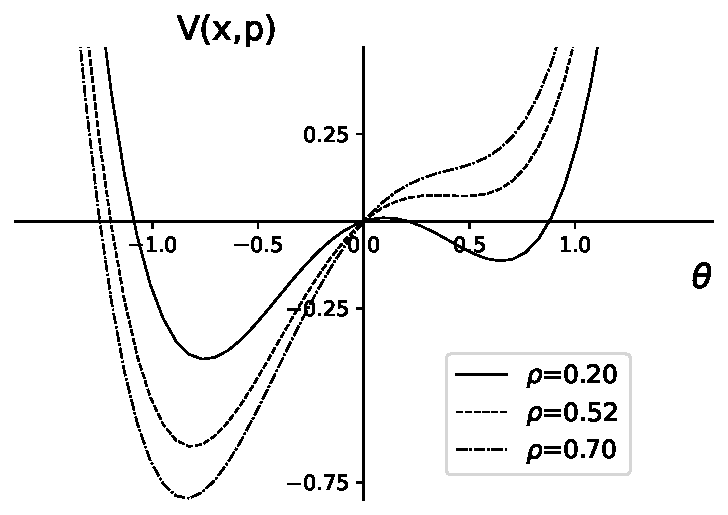
\includegraphics[width=\linewidth]{cat_mac_p_tilt}
		\renewcommand{\figurename}{Fig.}
	\end{minipage} 
	\caption{\small \textbf{Left:} The vector field is translated upwards under increasing $\rho$. Initially, three equilibria exist, then only two (of which one is stable and the other unstable). Finally, one equilibrium is destroyed and only one survivor hosts the system state. \textbf{Right:} the tilting parameter deforms to the potential as if it was tilted. One equilibrium goes from stability to instability and then disappears. Hence, any system state lying on the right branch will eventually transit critically towards the left-hand equilibrium. The process is exactly analogous to a fold bifurcation, Sec~\ref{subsec:fold}.}
	\label{fig:cm_tilting}
\end{figure}



\tocless\subsubsection{Combining parameters}
What happens, then, if we combine the effect of the two parameters? The potential, Eq. \ref{eq:cm_potential}, is bended and tilted at the same time (Fig. \ref{fig:cm_comb}), yielding a) asymmetric stable configurations (solid line), b) asymmetric bistable configurations (dashed), c) configurations with critical transitions happening at lower forcing $\rho$ than before (dash-dotted). In general, the two parameters combined set the degree of hysteresis of the system and the possibility of observing a critical transition.\\



\begin{figure}[h]
	\centering
	\begin{minipage}[c]{0.48\textwidth}
		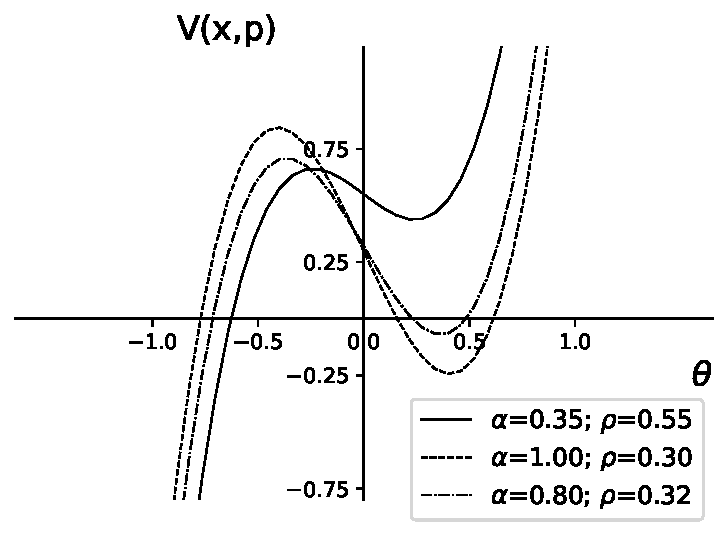
\includegraphics[width=\linewidth]{cat_mac_v_comb}
		\renewcommand{\figurename}{Fig.}
	\end{minipage}
	\hspace{0.05cm}
	\begin{minipage}[c]{0.48\textwidth}
		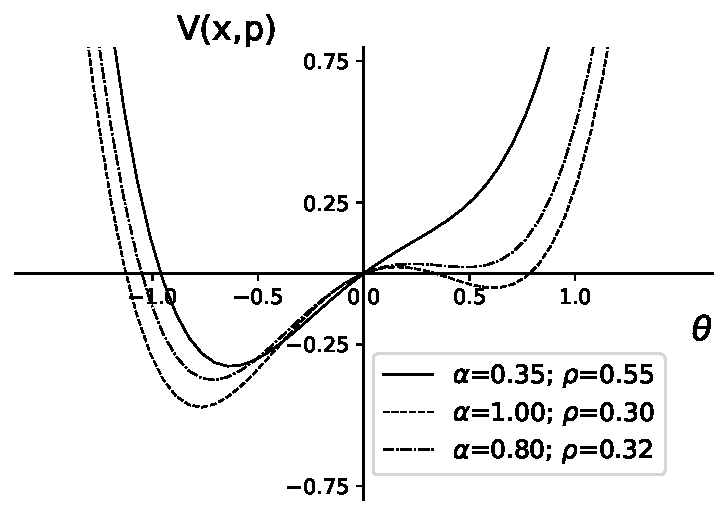
\includegraphics[width=\linewidth]{cat_mac_p_comb}
		\renewcommand{\figurename}{Fig.}
	\end{minipage} 
	\caption{\small \textbf{Left:} Different $f(\theta)$ coming from different parameter combinations.\textbf{Right:} different $V(\theta)$ associated with different parameter combinations. The shape of the potential (ruled by $\alpha$) is necessary to set the susceptibility of a system to tip, but the intersection with the zero axis is what drives the \gls{CT}. So, both parameters should be taken into account while studying similar systems. }
	\label{fig:cm_comb}
\end{figure}



\tocless\subsection{Analytical calculation}
Since the explicit potential is known, it is possible to analytically calculate the values for which the tipping happens, as well as the functional form of the parameters relationship leading to critical transitions.
The critical transition point is given by the intersection of the vector field manifold and of its tangent space. We can verify this fact in two ways:
\begin{enumerate}
	\item Formally, consider the unfolding of the associated bifurcation, and study its associated vector field. Look for steady states and their stability. From this, identify the fold point and the stability of the associated manifold \citep{kuehn2013mathematical}. The process is akin to solving the following system:
	\begin{equation}
		\begin{cases} f = 0 \\ D_x f|_{C_0} = 0 \end{cases} 
	\end{equation}
	where $C_0$ represents the fold manifold.
	
	\item Intuitively, we need to check when a minimum in the potential coalesces into a flexus point (this is the condition for indifferent equilibrium). Hence, the system to be solved is:
	\begin{equation}
		\begin{cases} \frac{dV}{dx} = 0 \\ \frac{d^2 V}{dx^2}|_{\hat{x}} = 0 \end{cases} 
		\label{solve}
	\end{equation}
	where the first equation finds the minima $\bar{x}$ and the second calculates a flexus point in the minima.
\end{enumerate}
Obviously, the two formulations are equivalent in $1D$ (our case) thanks to the equivalence of the derivate operator and the manifold algebra (and do not forget that, in $1D$, $\frac{dV}{dx}=f$).



\subsubsection{Critical Transition}
Let us assume that the system is already at a bistable configuration (set $\alpha = 1$ w.l.o.g.). Then, estimate the critical value of $\rho$ for which the system undergo a \gls{CT}. Let us solve Eq. \ref{solve}. In our case, 
\begin{equation}
	\begin{cases} 4\hat{x}^3 - 2\hat{x} + \rho = 0 \\ 12\hat{x}^2 - 2= 0 \, .\end{cases} 
\end{equation}
The solution is:
\begin{equation}
	\begin{cases} \hat{x}_{1,2}=\pm\left(\frac{1}{6} \right)^{1/2} \\ \rho_{CT}|_{\hat{x}_1} = \frac{4}{3}\left(\frac{1}{6}\right)^{1/2} \, . \end{cases} 
\end{equation}
$\hat{x}$ identifies the steady state points and $\rho_{CT}$ is the critical value of the parameter for which a critical transition occurs. Those values have no real quantitative meaning when compared to the actual machine, as the potential was already rescaled to avoid constant dependencies on empirical values; it is difficult to get them from an artisanal machine, unless under perfectly controlled conditions. Nonetheless, this depicts the general procedure to study critical values in a model.



\subsubsection{Rising bistability followed by Critical Transition}
When both parameters are considered, we have to look at combinations for which a CT happens. Hence, we search for a set $(\alpha, \rho)$ for which the system is bistable and tipping. There are two parameters to consider, so we can look at the reduced curve \citep{kuehn2013mathematical} defined by $\rho(\alpha)$. Following the same procedure as before, thus solving system \ref{solve} again, we eventually get, from $\hat{x}_1$:
\begin{equation}
	\rho = \left( \frac{2}{3}\alpha \right)^{\frac{3}{2}}
\end{equation}
as a solution. The other three solutions are given by $\hat{x}_2$ and by considering the case where $\theta \rightarrow \theta - \pi$ (corresponding to the opposite side of the pivot in the Catastrophe Machine). By plotting all four relationships $\rho = f(\alpha)$, we obtain the diamond-shaped plot shown in Fig. \ref{fig:cusptheo} (left). This is the hallmark of a cusp bifurcation, see Sec. \ref{subsec:cusp} and Fig. \ref{fig:cusp}, left. Fig. \ref{fig:cusptheo} (left) predicts the set of points (qualitatively speaking) that is obtained empirically by playing with the machine and by pinpointing with a pencil when it tips (see Fig. \ref{fig:cusptheo}, right).


\begin{figure}[h]
	\centering
	\begin{minipage}[c]{0.48\textwidth}
		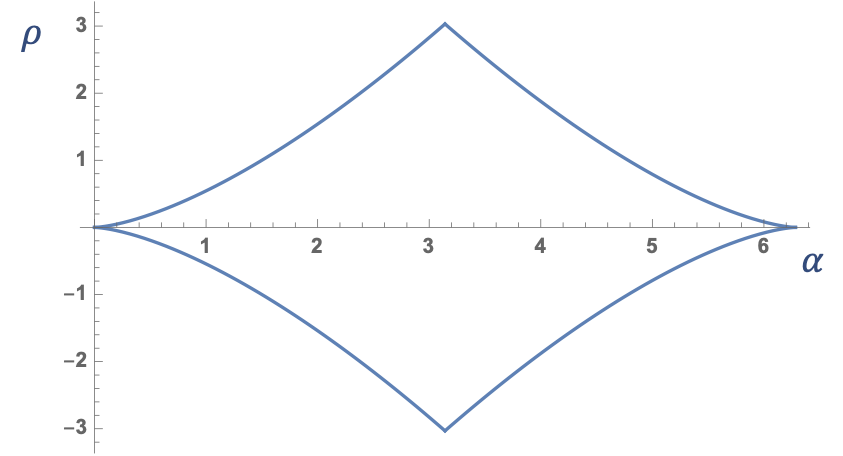
\includegraphics[width=\linewidth]{cusp}
		\renewcommand{\figurename}{Fig.}
	\end{minipage}
	\hspace{0.05cm}
	\begin{minipage}[c]{0.48\textwidth}
		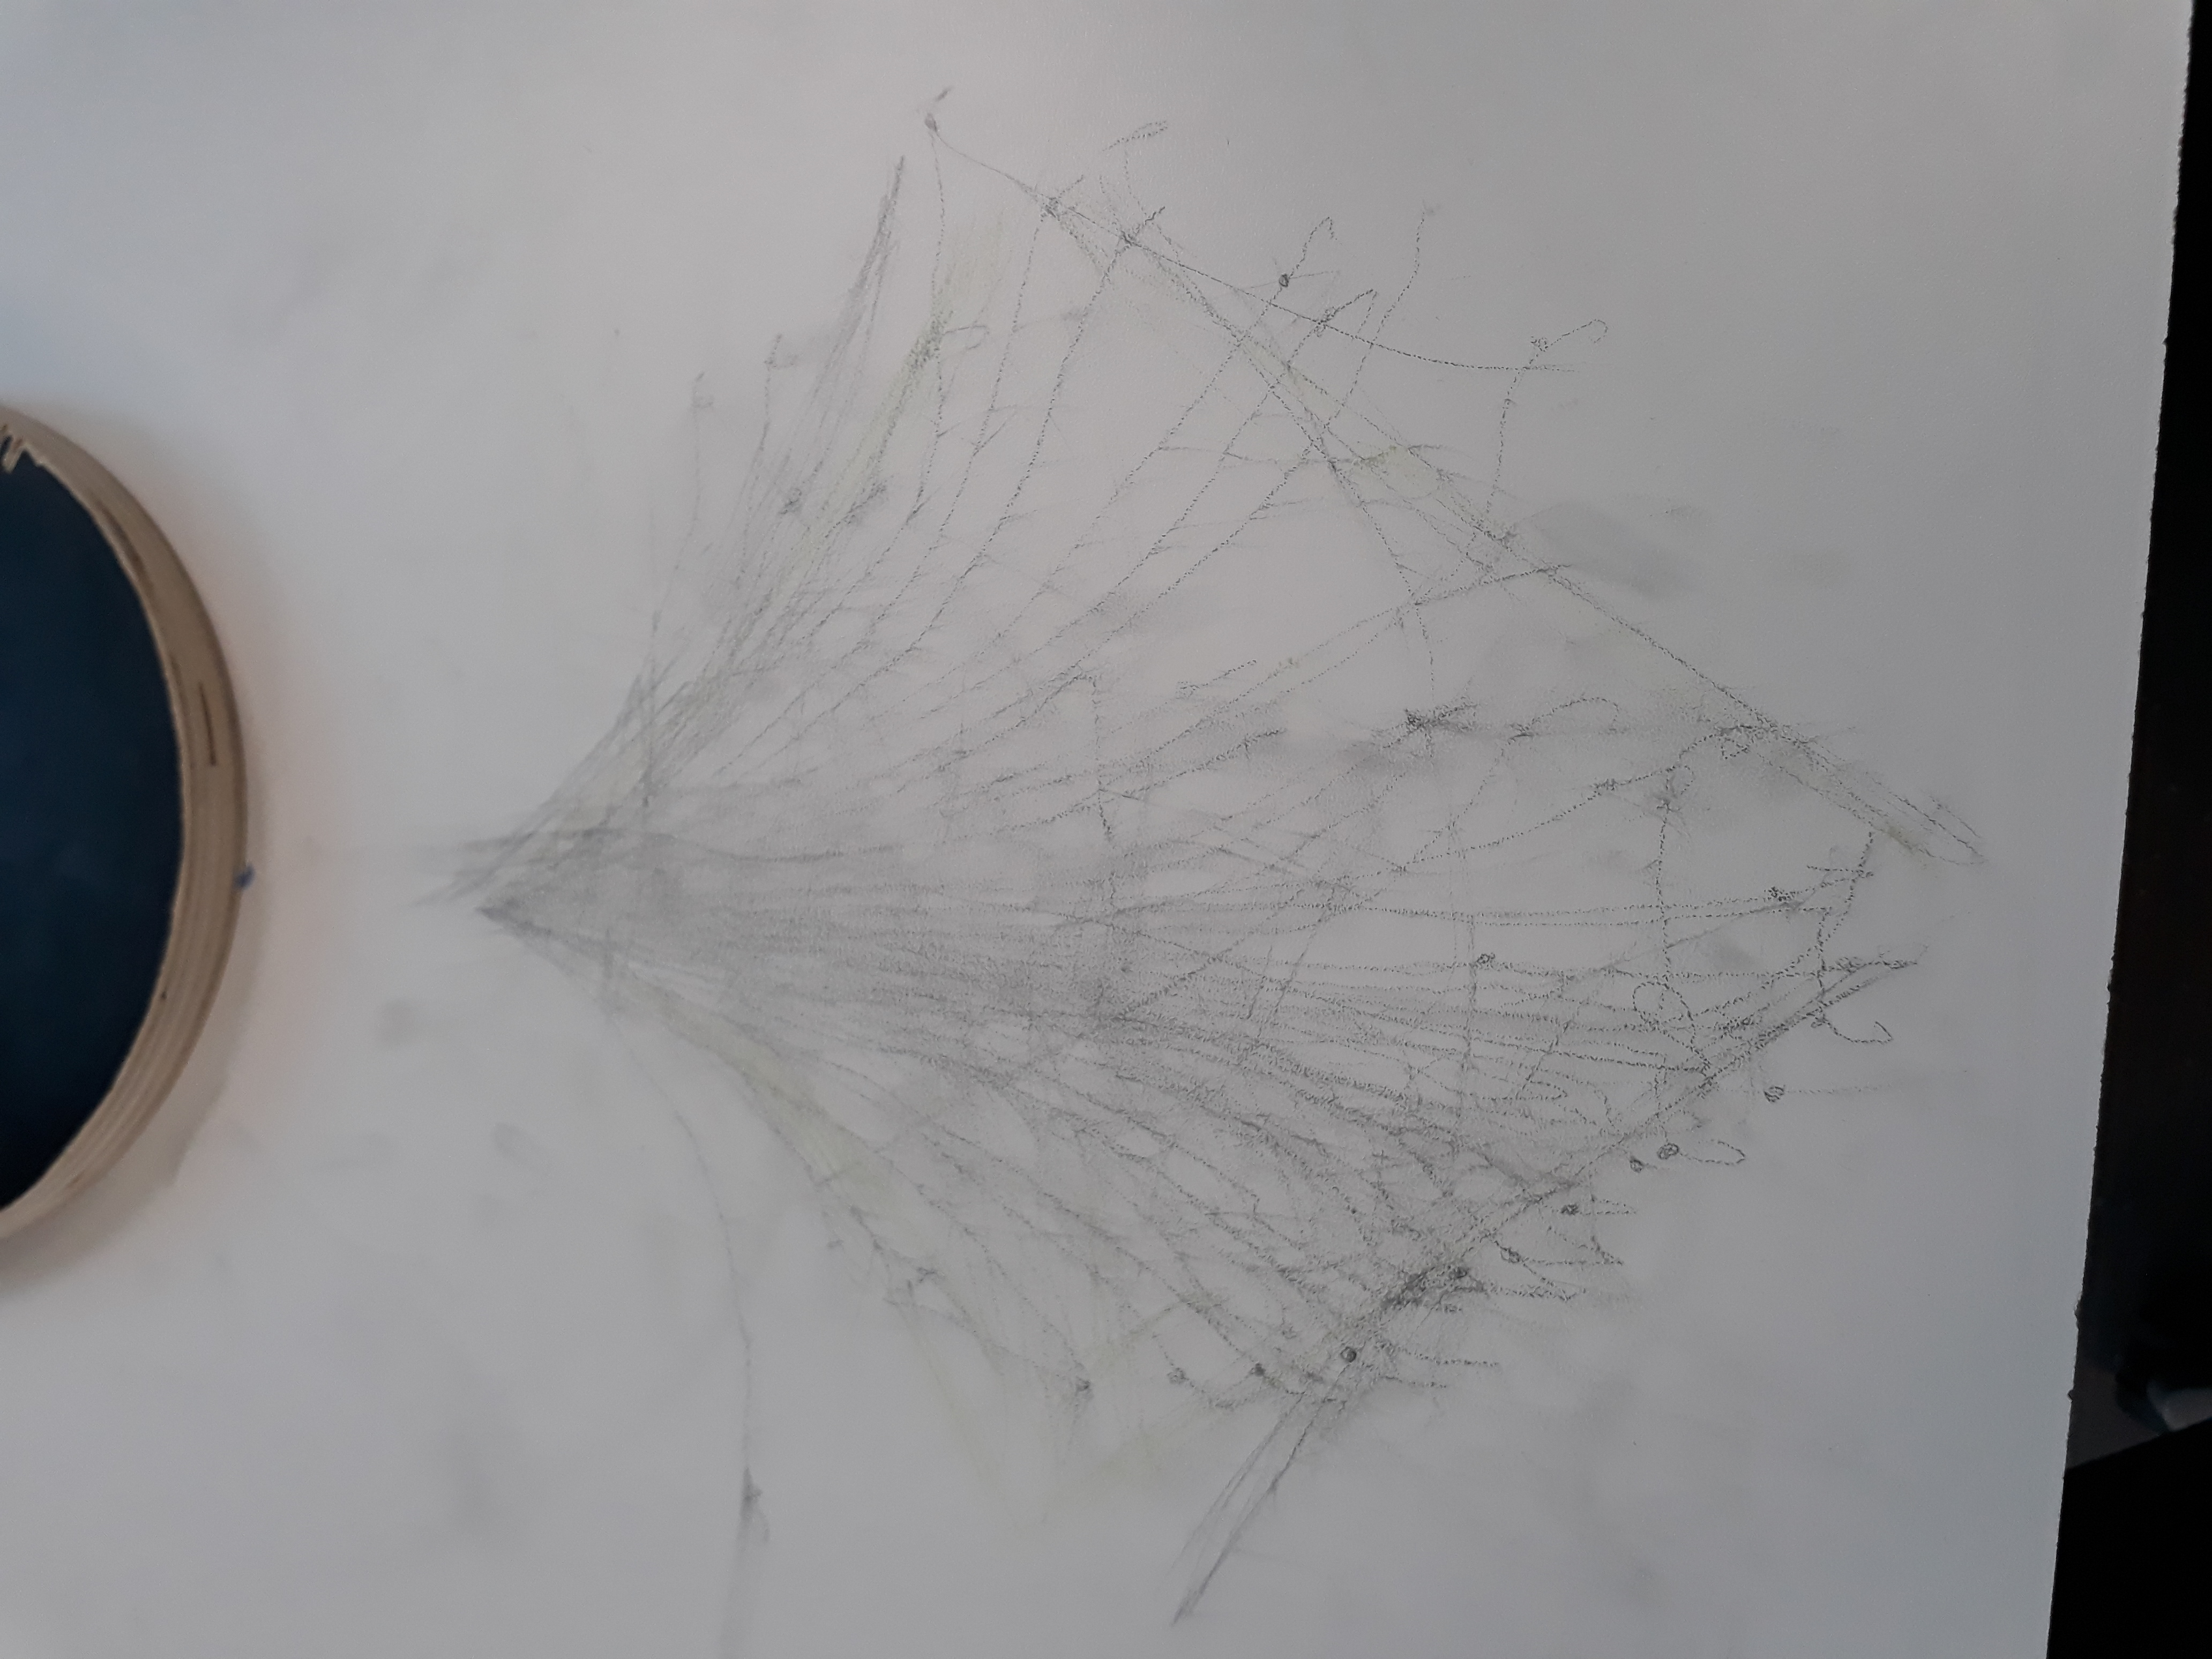
\includegraphics[width=0.8\linewidth]{cuspemp}
		\renewcommand{\figurename}{Fig.}
	\end{minipage} 
	\caption{\small \textbf{Left:} The shape of $\rho = f(\alpha)$.\textbf{Right:} The diamond-shaped drawing that was empirically obtained by following the tipping behaviour of the machine with a pencil. It is not perfectly symmetric because of the friction and of elastic properties. }
	\label{fig:cusptheo}
\end{figure}


Two side notes on the analysis just performed. First, I wrote ``qualitative'' for the following reason: we are asking ``does the machine exhibits CT? If so, under which conditions?'' rather than ``What is the exact value of the forcing after which the machine tips over''? Second, the present analysis was possible thanks to an available mechanistic model, developed from first principles of Newtonian dynamics. On the other hand, it might not be conclusive to observe a diamond shape on a board and infer that it was produced by a potential like \ref{eq:cm_potential}.


\tocless\section{Limitations and challenges}

Limitations: the catastrophe machine can be analysed thoroughly thanks first principles yielding a closed-form potential. Then, the emphasis on the two parameters controlling the system inscribes this study on the theory of catastrophes \citep{Thom2554}, that works fine for those systems whose potential is known. On the other hand, as several authors pointed out \citep{Zahler1977,kolata1977catastrophe}, it is not fruitful nor informative to speculate about the existence of such potential in any system that behaves vaguely similarly. It is the proponent who, in principle, should  have the burden of proof, starting from experiments ad developing models. Using Catastrophe Theory as a mathematics-based philosophy could be misleading, as it detaches the modelling attempts from the experimental practice. On the other hand, such theory - and the Catastrophe Machine in particular - has already proven to be useful in controlled contexts and as an heuristic guide for experiments and speculation (hypothesis formulation). Further developments will also include diminishing the friction and coupling two wheels to obtain a chaotic behavior \citep{nagy2013zeeman}. The latter case, which was initiated with a new machine (Fig. \ref{fig:newcat}) but was not further studied during the PhD period, will help to assess conditions for chaoticity rising from coupled nonlinear systems.

\begin{figure}[h!]
	\centering
	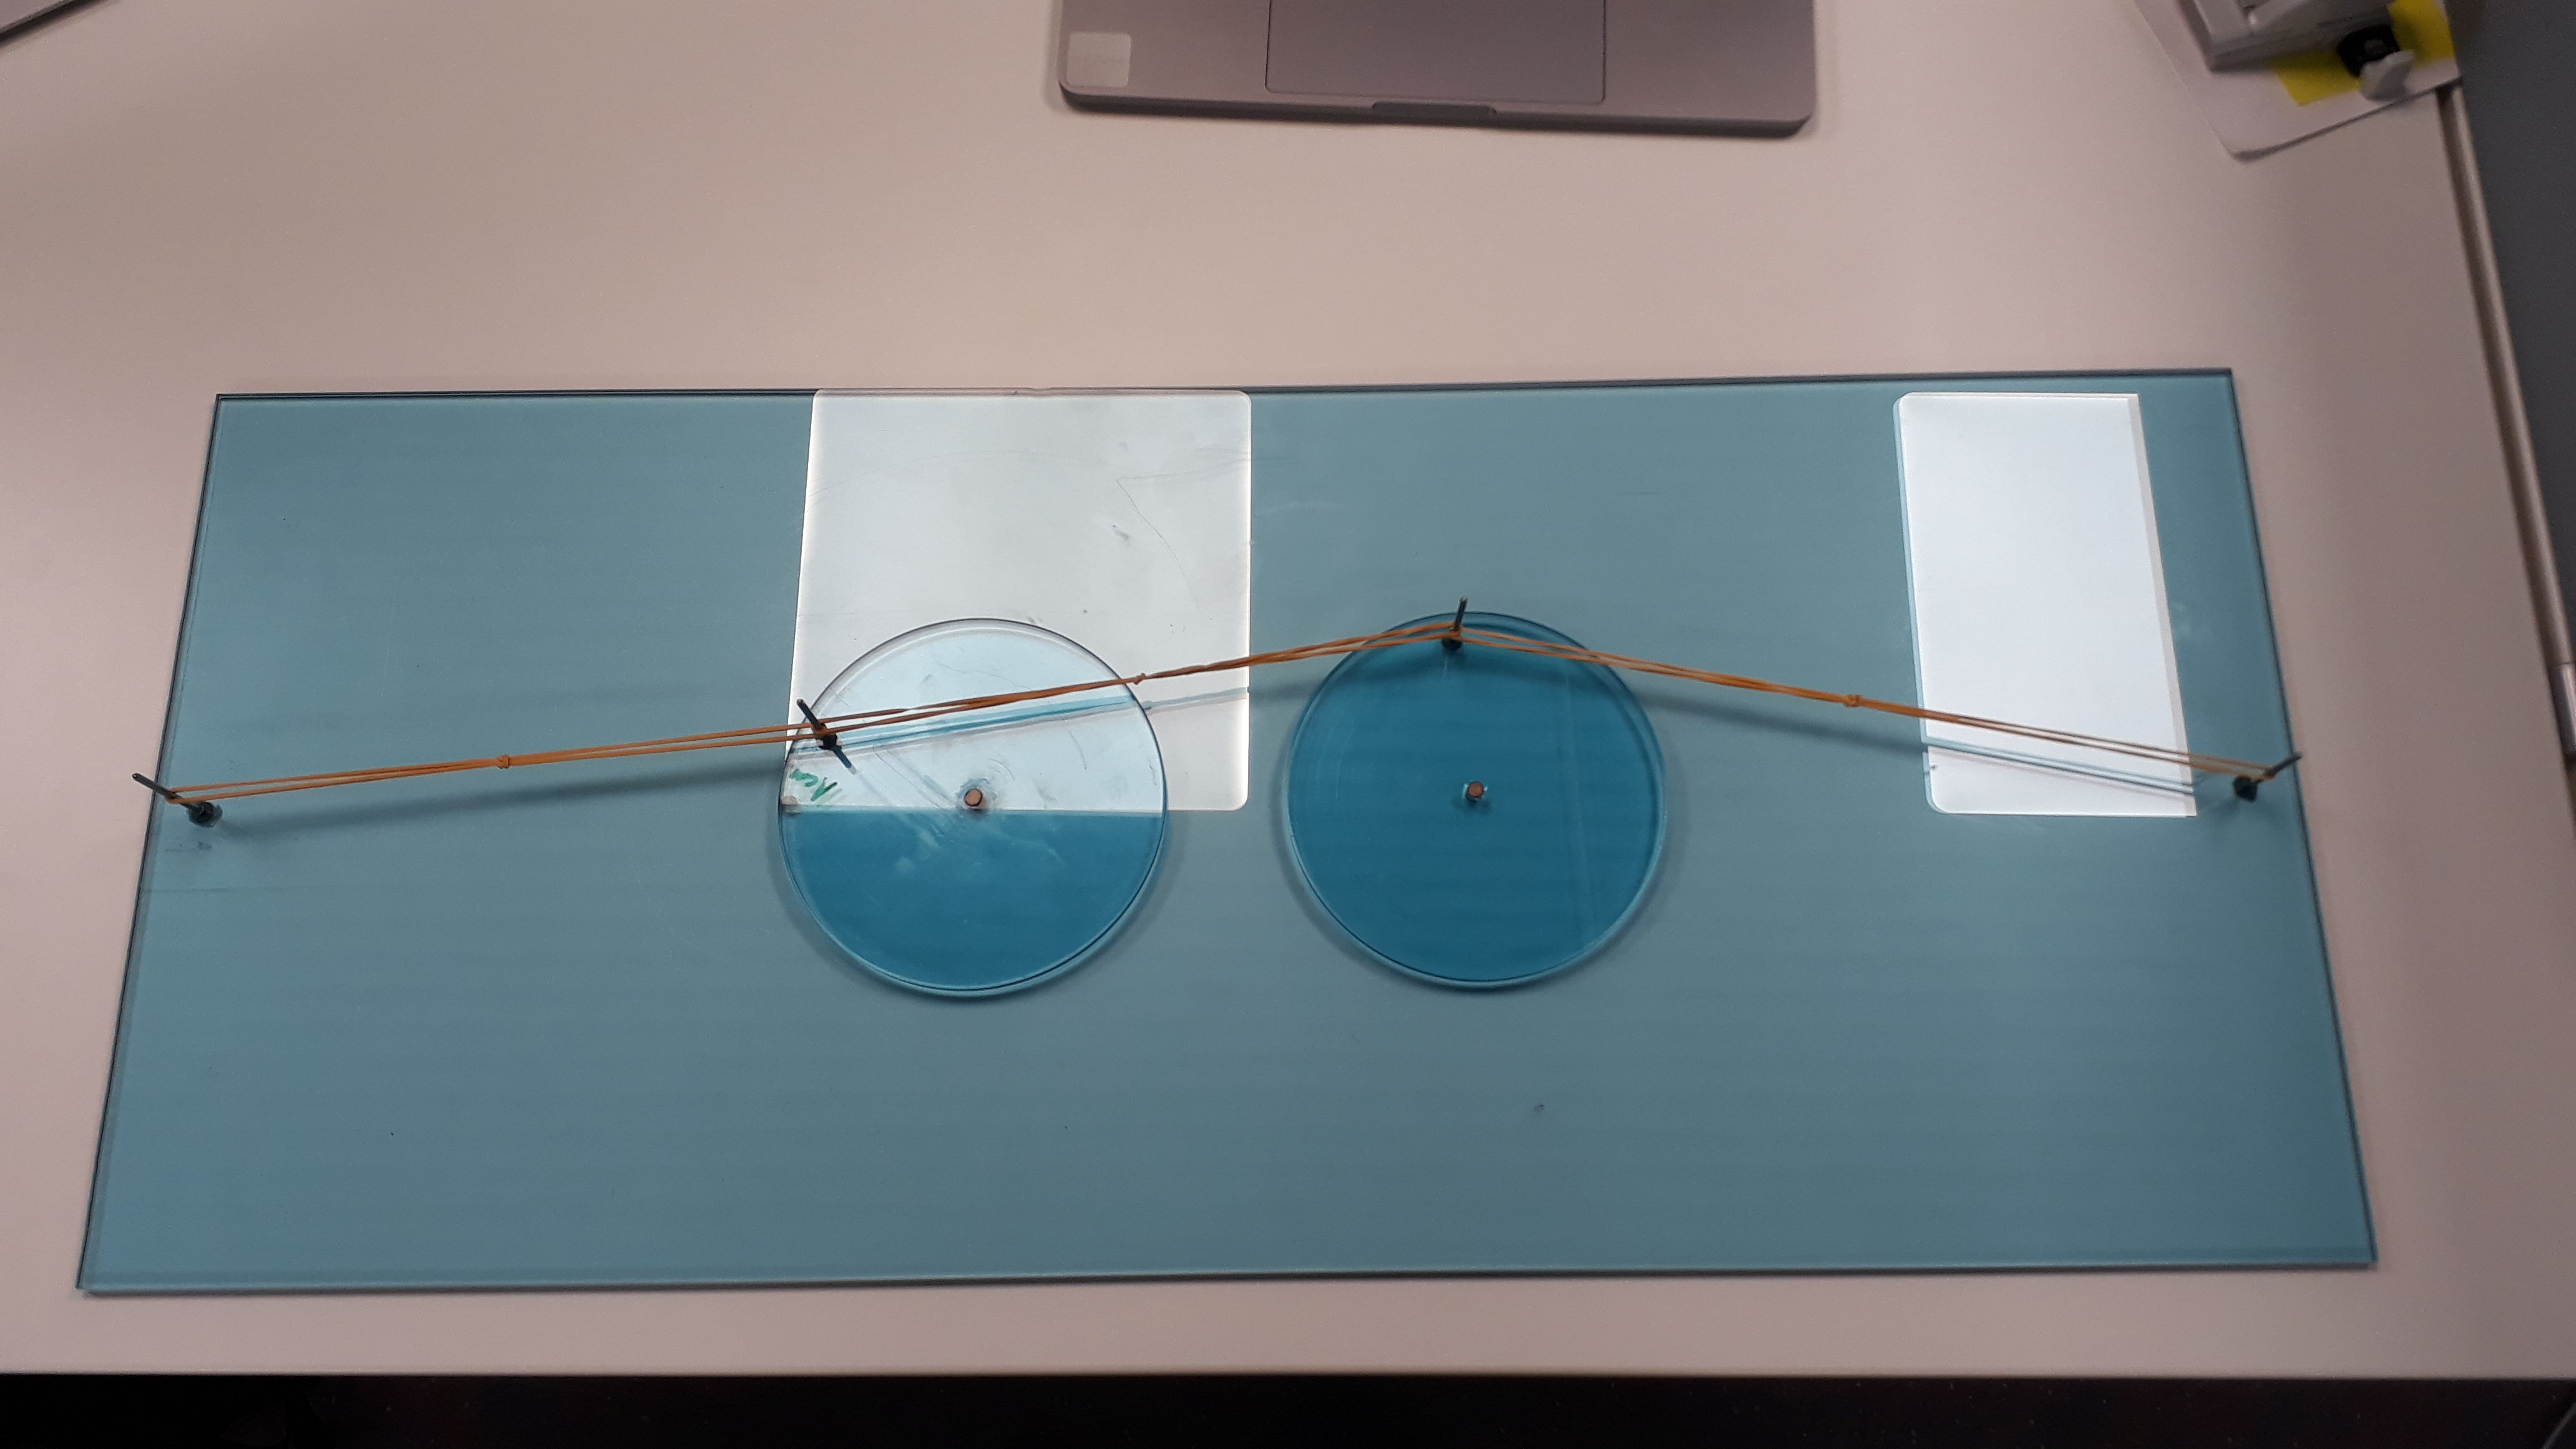
\includegraphics[width=0.6\linewidth]{new_cat}
	\caption{\small The upgraded Catastrophe Machine. It consists of two wheels, with increased distance from the pivots (to make the infinity approximation better), of which one can be adjusted in different positions. Moreover, friction was consistently reduced thanks to the material (plastic instead of wood).}
	\label{fig:newcat}
\end{figure}

